\documentclass[twoside,11pt]{Latex/Classes/PhDthesisPSnPDF}
% This file contains macros that can be called up from connected TeX files
% It helps to summarise repeated code, e.g. figure insertion (see below).

% insert a centered figure with caption and description
% parameters 1:filename, 2:title, 3:description and label
\newcommand{\figuremacro}[3]{
	\begin{figure}[htbp]
		\centering
		\includegraphics[width=1\textwidth]{#1}
		\caption[#2]{\textbf{#2} - #3}
		\label{#1}
	\end{figure}
}

% insert a centered figure with caption and description AND WIDTH
% parameters 1:filename, 2:title, 3:description and label, 4: textwidth
% textwidth 1 means as text, 0.5 means half the width of the text
\newcommand{\figuremacroW}[4]{
	\begin{figure}[htbp]
		\centering
		\includegraphics[width=#4\textwidth]{#1}
		\caption[#2]{\textbf{#2} - #3}
		\label{#1}
	\end{figure}
}

% inserts a figure with wrapped around text; only suitable for NARROW figs
% o is for outside on a double paged document; others: l, r, i(inside)
% text and figure will each be half of the document width
% note: long captions often crash with adjacent content; take care
% in general: above 2 macro produce more reliable layout
\newcommand{\figuremacroN}[3]{
	\begin{wrapfigure}{o}{0.5\textwidth}
		\centering
		\includegraphics[width=0.48\textwidth]{#1}
		\caption[#2]{{\small\textbf{#2} - #3}}
		\label{#1}
	\end{wrapfigure}
}

% predefined commands by Harish
\newcommand{\PdfPsText}[2]{
  \ifpdf
     #1
  \else
     #2
  \fi
}

\newcommand{\IncludeGraphicsH}[3]{
  \PdfPsText{\includegraphics[height=#2]{#1}}{\includegraphics[bb = #3, height=#2]{#1}}
}

\newcommand{\IncludeGraphicsW}[3]{
  \PdfPsText{\includegraphics[width=#2]{#1}}{\includegraphics[bb = #3, width=#2]{#1}}
}

\newcommand{\InsertFig}[3]{
  \begin{figure}[!htbp]
    \begin{center}
      \leavevmode
      #1
      \caption{#2}
      \label{#3}
    \end{center}
  \end{figure}
}


%%% Local Variables: 
%%% mode: latex
%%% TeX-master: "~/Documents/LaTeX/CUEDThesisPSnPDF/thesis"
%%% End: 

\usepackage{microtype}
\usepackage{graphicx}
\usepackage{wrapfig}
\usepackage{fancyhdr}
\usepackage{amsmath}
\usepackage{titlesec}
\usepackage{tabularx}
\usepackage{booktabs}
\usepackage{subcaption}


\usepackage{color}\usepackage{graphicx,xcolor}
\usepackage[margin=3.5cm]{geometry}
\setcitestyle{square}


\usepackage{hyperref}
\hypersetup{
    colorlinks, % set true if you want colored links
    citecolor=black,
    filecolor=black,
    linkcolor=blue, % choose some color if you want links to stand out
    urlcolor=black
}

\usepackage[figurename=Figura]{caption}
\usepackage[tablename=Tabla]{caption}


%: ----------------------------------------------------------------------
%:                      Título, nombre, logo...
% ----------------------------------------------------------------------
%Clasificador mediante imágenes de cáncer de piel
\title{%
  CLASIFICADOR \\ MEDIANTE IMÁGENES DE \\ CÁNCER DE PIEL \\
  \large
  \bigskip 
  %FACULTAD DE INGENIERÍA INFORMÁTICA
  Facultad de Ingeniería Informática \\
  Departamento de Informática y Sistemas}

\ifpdf
  \author{\href{prashantjeswani8@gmail.com}{Prashant Jeswani Tejwani}}
  \collegeordept{Bajo la dirección del doctor \\
                José María Quinteiro González}
                
  \university{\href{https://www.ulpgc.es/}{Universidad de Las Palmas de Gran Canaria}}

  % The crest is a graphics file of the logo of your research institution.
  % Place it in ./0_frontmatter/figures and specify the width
  
  \crest{
\includegraphics[width=14cm]{0_frontmatter/figures/LogoEII.jpg}}
\fi

\renewcommand{\submittedtext}{Memoria para optar al}
\degree{Grado de Ingeniería Informática}
\degreedate{Las Palmas de Gran Canaria, 2021}

% Turn of those nasty overfull and underfull hboxes
\hbadness=10000
\hfuzz=50pt

\begin{document}
% Sets line spacing
\renewcommand\baselinestretch{1.2}
\baselineskip=18pt plus1pt


%: --------------------------------------------------------------
%:                  Frontpage, abstract, acknowledgement
% --------------------------------------------------------------
\maketitle  % title page
\newgeometry{margin=1.5cm}

\pagestyle{empty}

%\lhead{ 
\begin{tabular}{p{15cm}p{5cm}}
  
\includegraphics{0_frontmatter/figures/LogoEII.jpg}   &  TFT04\\
\end{tabular}
%}

\vspace{1em}
\fboxrule=2pt
\begin{center}
\fcolorbox{gray}{gray!10}{\parbox{.65\textwidth}{ {\large SOLICITUD DE DEFENSA DE TRABAJO DE FIN DE TÍTULO}}}
\end{center}

\vspace{1em}
\justify
D./Dª \underline{Prashant Jeswani Tejwani}, autor del Trabajo de Fin de Título \underline{Clasificador mediante imágenes de}

\underline{cáncer de piel}, correspondiente a la titulación Grado de Ingeniería Informática.

\vspace{1em}
SOLICITA

\vspace{1em}
que se inicie el procedimiento de defensa del mismo, para lo que se adjunta la documentación requerida, haciendo constar que 
\vspace{1em}

\hspace{10mm} [X] se autoriza / [ ] no se autoriza la grabación en audio de la exposición y turno de preguntas.

\vspace{1em}
Asimismo, con respecto al registro de la propiedad intelectual/industrial del TFT, declara que:
\vspace{1em}

\hspace{10mm} [ ] Se ha iniciado o hay intención de iniciarlo (defensa no pública).

\hspace{10mm} [X] No está previsto.

\vspace{1em}
Y para que así conste firma la presente. 

\begin{center}
En Las Palmas de Gran Canaria, a 26 de octubre de 2021

\vspace{1em}
El estudiante

\vspace{3em}
Fdo.------------------------
\end{center}

\begin{center}

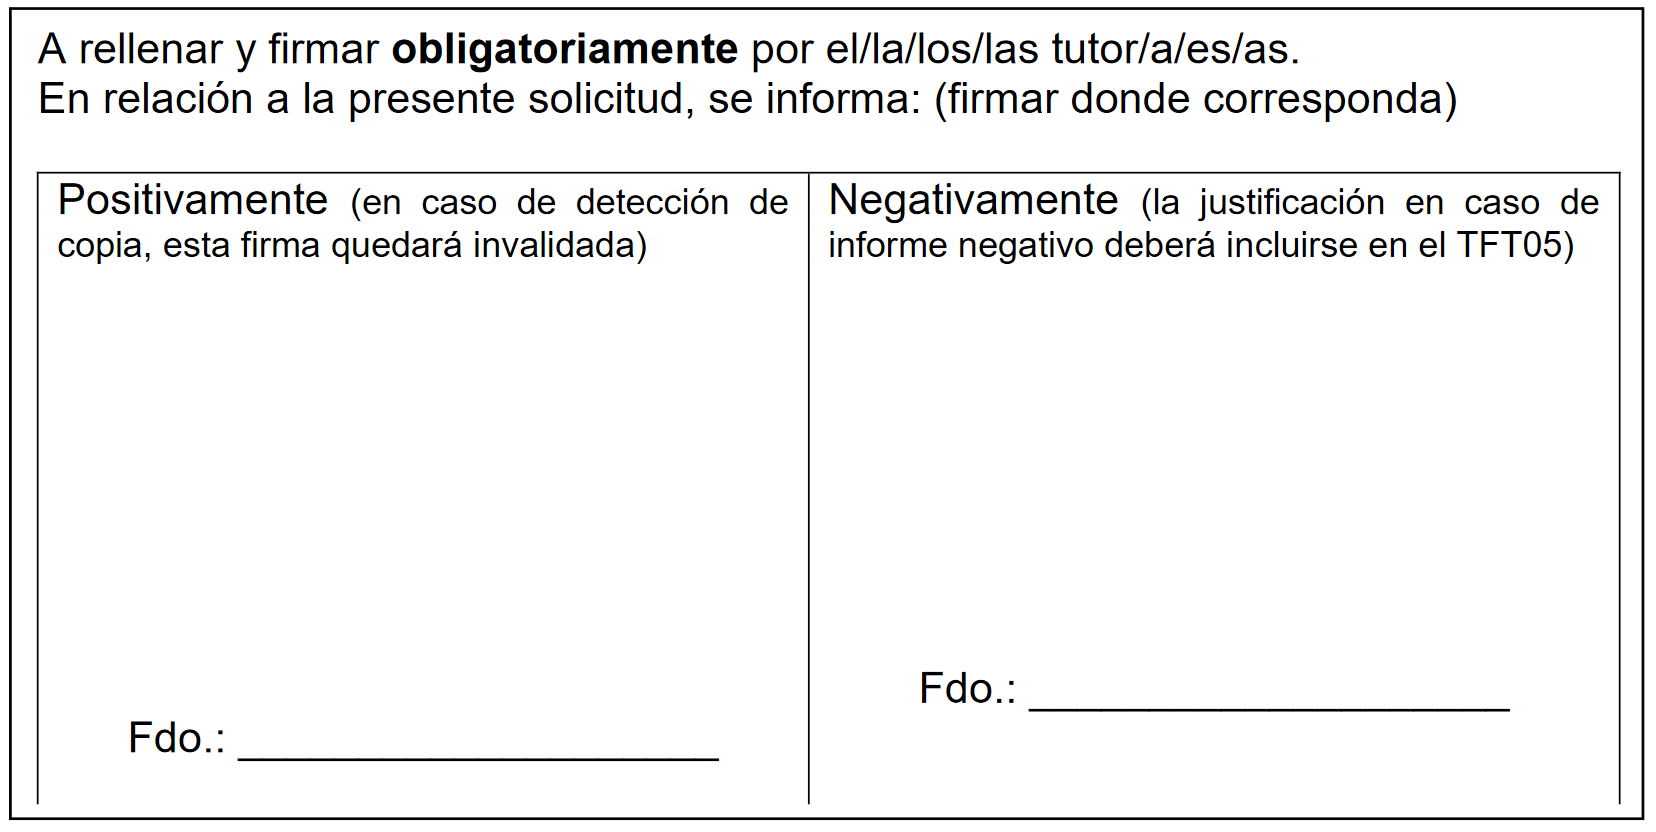
\includegraphics[scale=0.6]{0_frontmatter/figures/firmasTFT04.PNG}

%\fcolorbox{gray}{white!10}{\parbox{.75\textwidth}{
%A rellenar y firmar \textbf{obligatoriamente} por %el/la/los/las tutor/a/es/as.

%En relación con la presente solicitud, se informa:

%\vspace{1em}
%\begin{tabular}{lr}
  %[X] Positivamente  & [ ] Negativamente (justificación %en TFT05)\\
%\end{tabular} 

%\vspace{3em}
%\center{Fdo.------------------------ }
%
%}}

\vspace{1em}

%\cfoot{
DIRECTOR DE LA ESCUELA DE INGENIERÍA INFORMÁTICA
%}

\end{center}

\restoregeometry % TFT04
\begin{abstracts}

Las decisiones médicas son difíciles ya que menudo deben tomarse con información insuficiente e incierta. Además, el resultado del proceso de decisión tiene implicaciones de gran alcance en el bienestar humano o incluso vidas. 

El desempeño humano en la toma de decisiones disminuye con la complejidad de los problemas y la presión del tiempo. Por lo tanto, el apoyo de médicos a la toma de decisiones es crucial, especialmente en su fase inicial cuando un especialista debe elaborar un diagnóstico preliminar y especificar las posibles direcciones para el tratamiento del paciente.

Las herramientas informáticas tienen el potencial de marcar la diferencia en la medicina. Especialmente las redes profundas, que pueden aprovechar tanto el gran número de datos disponibles como la experiencia clínica.

La aplicación de redes profundas al diagnóstico se ha propuesto hace casi dos décadas, teniendo potencial para beneficiar significativamente la atención médica. Sin embargo, la difusión práctica de este enfoque sigue siendo mínima.

El objetivo de este trabajo es introducir un clasificador de diagnóstico de cáncer de piel basado en redes bayesianas utilizando Monte Carlo Dropout, propuesta por Gal \& Ghahramani en 2016 \cite{bayesian_networks-gal}. Se realiza comparaciones con varios modelos, además de mostrar otras formas de hacer frente los datos desbalanceados en datos clínicos frente a las técnicas clásicas. También se muestra la conveniencia de calibrar los modelos de clasificación para que las probabilidades mostradas en el diagnóstico se ajusten a los datos.

Finalmente, se argumenta que un diagnóstico con la ayuda informática puede ser beneficiosa para sus usuarios y mejorar la precisión diagnóstica de los médicos.

\end{abstracts}
 % abstract

\frontmatter
%%\begin{acknowledgementslong} %uncommenting this line, gives a different acknowledgements heading
\begin{acknowledgements}      %this creates the heading for the acknowlegments

I would like to acknowledge the thousands of individuals who have coded for the LaTeX project for free. It is due to their efforts that we can generate professionally typeset PDFs now.

\end{acknowledgements}
%\end{acknowledgmentslong}


 % acknowledgement


%: --------------------------------------------------------------
%:                  Contents, list of figures/tables
% --------------------------------------------------------------
\setcounter{secnumdepth}{3} % organisational level that receives a numbers
\setcounter{tocdepth}{3} % print table of contents for level 3
\renewcommand{\contentsname}{Índice de contenido}
\renewcommand{\listfigurename}{Índice de figuras}
\renewcommand{\listtablename}{Índice de tablas}
\tableofcontents 
\listoffigures
\listoftables  


%: --------------------------------------------------------------
%                           MAIN DOCUMENT
% --------------------------------------------------------------
\mainmatter
\renewcommand{\chaptername}{} % uncomment to print only "1" not "Chapter 1"

\section{Introducción}
El cáncer de piel es una enfermedad de carácter más o menos grave, según el tipo de tumor al que dé lugar. \\
El melanoma es un tipo de cáncer de piel que se origina cuando los melanocitos (las células responsables de la pigmentación normal de la piel) comienzan a crecer fuera de control. El melanoma es mucho menos frecuente que otros tipos de cánceres de piel, aunque es el más peligroso y agresivo porque evoluciona muy rápidamente, es de fácil diseminación por el organismo y muchas veces mortal si no es detectado en una fase temprana. 
\bigskip

\begin{figure}[htbp]
    \centering
    \textbf{}\par\medskip
    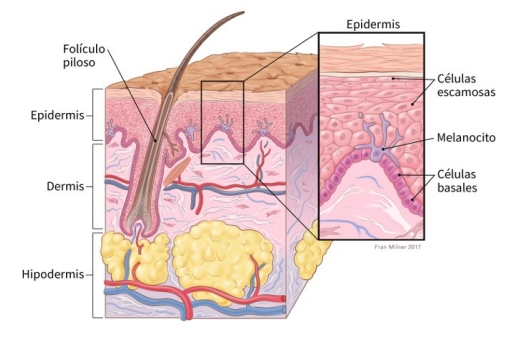
\includegraphics[scale=0.70]{figures/skin.png}
    \caption{Capas de la piel}
\end{figure}

\pagestyle{fancy}
\fancyhf{}
\fancyhead[L]{1. INTRODUCCIÓN}
\newpage
Muchos tipos de tumores benignos (no cancerosos) se pueden originar de los diferentes tipos de células de la piel. Un lunar es un tumor benigno de la piel que también se origina a partir de los melanocitos. No obstante, casi todos los lunares son inofensivos, aunque algunos tipos pueden aumentar su riesgo de melanoma. \\
Un tipo de lunar que a veces se parece al melanoma se llama “nevo Spitz”. Este lunar es más común en niños y adolescentes, aunque a veces se presenta en adultos. Por lo general, estos tumores son benignos y no se propagan. Sin embargo, en ocasiones los médicos tienen problemas para distinguir entre un “nevo Spitz” y un melanoma, aun cuando los observan con un microscopio.

En general, las variedades de melanoma se caracterizan por su Asimetría, Borde irregular, Color heterogéneo, Diámetro grande ($<$ 6mm) y Evolución rápida, también conocido como la regla del ABCDE.
Se reconocen actualmente como factores de riesgo de melanoma: 
\bigskip

\begin{tabular}{|cl|cl|}
TABLA DE CAUSAS
\end{tabular}

\bigskip
Según la etapa del cáncer y otros factores, las opciones de tratamiento podrían incluir: cirugía, inmunoterapia, medicamentos de terapia, quimioterapia, radioterapia para el cáncer de piel tipo melanoma, entre otros.

\chapter{Diagnosis en \\ Hematología/Oncología}
La Hematología/Oncología es la rama de la medicina que se centra en el diagnóstico y tratamiento de numerosos trastornos sanguíneos, incluidos el cáncer, la anemia, la leucemia y la enfermedad de Hodgkin, y el diagnóstico y tratamiento de cánceres y tumores benignos y malignos.

La mejor manera de detectar el melanoma es examinando continuamente la piel de los pacientes, especialmente los lunares. Una llaga, una protuberancia o un tumor en la piel también puede ser un signo de melanoma u otro cáncer de piel. El melanoma se puede encontrar en varios lugares incluyendo la espalda, las nalgas, las piernas, el cuero cabelludo, el cuello, detrás de la oreja, las plantas de los pies, las palmas de las manos, dentro de la boca, los genitales y debajo de las uñas \cite{utmedicalcenter}. 

Según la Academia Americana de Dermatología (AAD), aproximadamente del 20\% al 40\% de los melanomas se desarrollan a partir de un lunar. Una llaga o tumor que sangra o cambios en el color de la piel también puede ser un signo de cáncer de piel \cite{utmedicalcenter}. 

%\newpage

La clave para tratar con éxito el melanoma es reconocer los síntomas a tiempo. Se recomienda realizar exámenes corporales anuales por un dermatólogo y examinarse la piel una vez al mes. Además, si un paciente ha tenido cáncer de piel, debe hacerse chequeos regulares para que un médico pueda examinar su piel.
Hay un número de pruebas que se pueden ordenar para diagnosticar el cáncer de piel: 

\begin{itemize}
\item Biopsia
\item Tomografía computarizada (TC)
\item Imagen de resonancia magnética (IRM)
\item Tomografía por emisión de positrones (TEP)
\end{itemize}

Por lo que un clasificador que sea capaz de discernir entre imágenes de piel de cáncer maligno y benigno ayudaría al diagnóstico mensual que deben hacer los médicos a sus pacientes además de reconocer los síntomas a tiempo.
\chapter{Conjunto de datos} 

Se ha hecho uso de un conjunto de datos generados por la International Skin Imaging Collaboration (ISIC) en donde las imágenes provienen de las siguientes fuentes: Hospital Clínic de Barcelona, Medical University of Vienna, Memorial Sloan Kettering Cancer Center, Melanoma Institute Australia, University of Queensland y University of Athens Escuela de Medicina \citep{isic-archive}.

Este conjunto de datos contiene 33.126 imágenes de entrenamiento dermatoscópicas de lesiones cutáneas benignas y malignas únicas de más de 2.000 pacientes. Cada imagen se asocia con una de estas personas mediante un identificador de paciente único. Todos los diagnósticos malignos se han confirmado mediante histopatología, y los diagnósticos benignos se han confirmado mediante el acuerdo de expertos, el seguimiento longitudinal o la histopatología. 

El conjunto de datos fue seleccionado para el SIIM-ISIC Melanoma Classification Challenge organizado en Kaggle durante el verano de 2020 \cite{kaggle}.


\section{Análisis de datos}

Las imágenes se proporcionan en formato DICOM, JPEG y TFRecord. Los metadatos también se proporcionan en archivos CSV.

\begin{figure}[htbp]
    \centering
    \textbf{}\par\medskip
    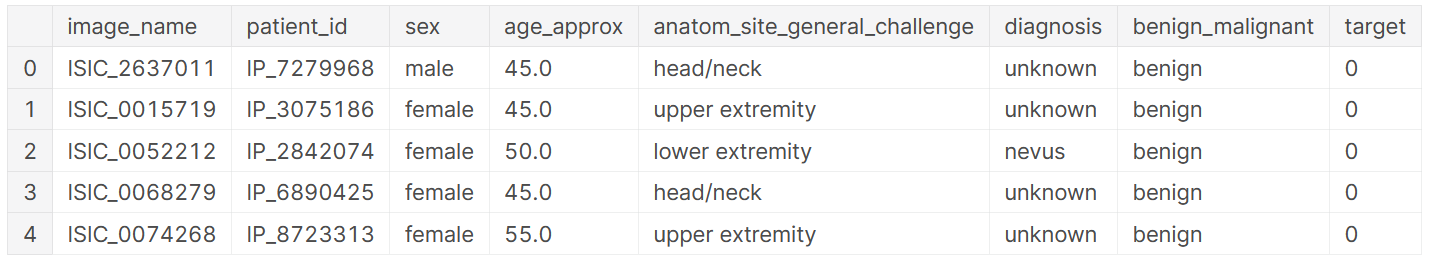
\includegraphics[scale=0.5]{3/figures/metadata/datos_tabulares.PNG}
    \caption{Primeras cinco filas de los datos tabulares de entrenamiento}
    \label{tabular_data}
\end{figure}

El propósito de la competición consiste en predecir un objetivo binario para cada imagen. El modelo debe predecir la probabilidad entre 0.0 y 1.0 de que la lesión en la imagen sea maligna. En los datos de entrenamiento, "train.csv", el valor 0 denota benigno y 1 indica maligno.

\begin{figure}[htbp]
    \centering
    \textbf{}\par\medskip
    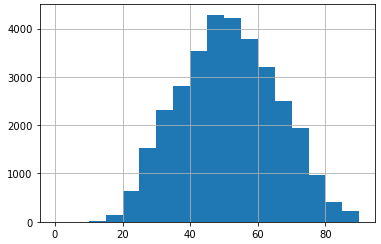
\includegraphics[scale=0.65]{3/figures/metadata/age_count.PNG}
    \caption{Edades}
    \label{age_count}
\end{figure}

\begin{figure}[htbp]
    \centering
    \textbf{}\par\medskip
    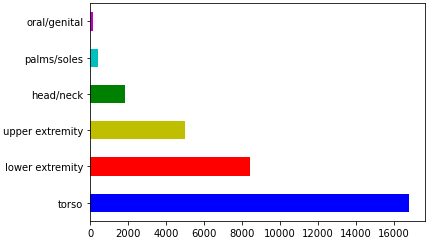
\includegraphics[scale=0.65]{3/figures/metadata/anatom_site_general_count.PNG}
    \caption{Parte del cuerpo}
    \label{anatom_site_general_count}
\end{figure}

\begin{figure}[htbp]
    \centering
    \textbf{}\par\medskip
    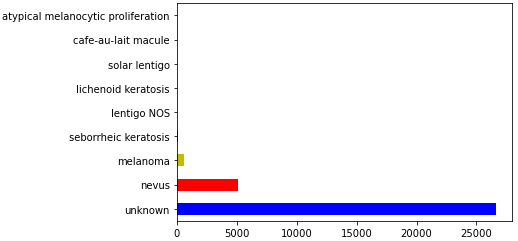
\includegraphics[scale=0.65]{3/figures/metadata/diagnosis_count.PNG}
    \caption{Diagnosis}
    \label{diagnosis_count}
\end{figure}

\begin{figure}[htbp]
    \centering
    \textbf{}\par\medskip
    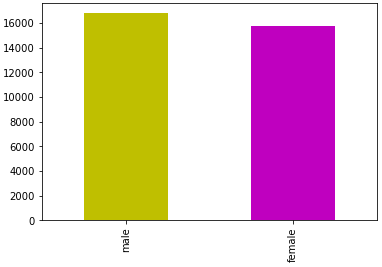
\includegraphics[scale=0.65]{3/figures/metadata/gender_count.PNG}
    \caption{Género}
    \label{gender_count}
\end{figure}

\begin{figure}[htbp]
    \centering
    \textbf{}\par\medskip
    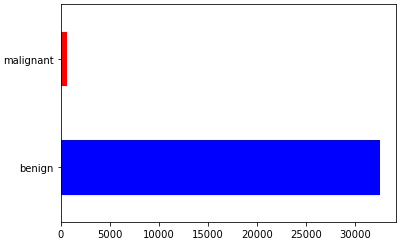
\includegraphics[scale=0.65]{3/figures/metadata/imbalance_class.PNG}
    \caption{Desbalanceo de clases}
    \label{imbalance_class}
\end{figure}

%\newpage

\subsection{Desbalanceo de datos}

La mayoría de los modelos utilizados para aprender de un conjunto de datos de las métricas utilizadas para evaluar esos modelos se diseñaron en torno al supuesto que la distribución de las clases sea igual. En cambio, cuando estas están desequilibrados, muchos algoritmos de aprendizaje automático fallan y las métricas utilizadas para evaluar esos modelos, como la precisión de la clasificación (o \emph{accuracy}), se vuelven engañosos \cite{imbalanced-classification}.

Como se observa en la figura \ref{imbalance_class}, existe un problema donde la distribución de ejemplos en las clases conocidas no está balanceada. Esto hace que la clase minoritaria sea más difícil de predecir porque hay pocos ejemplos de esta clase, por definición. Esto significa que es más difícil para un modelo aprender las características de los ejemplos de esta clase, y para diferenciar ejemplos de esta clase de la clase mayoritaria.

Como consecuencia, la mayoría de los modelos tienen un rendimiento predictivo deficiente, específicamente para la clase minoritaria. Esto presenta un inconveniente ya que la clase minoritaria (cáncer maligno) es más importante de clasificar correctamente y, por lo tanto, el problema es más sensible a los errores de clasificación para la clase minoritaria que la clase mayoritaria.


Para intentar solucionar este problema, se han propuesto modificaciones a los algoritmos existentes para hacer que sean útiles para la clasificación desequilibrada, la selección de métricas de rendimiento y nuevas técnicas de preparación de datos y algoritmos de modelado.

\subsubsection{Data augmentation}
Un enfoque para abordar los conjuntos de datos desequilibrados es sobremuestrear la clase minoritaria en el conjunto de datos de entrenamiento antes de entrenar el modelo. Esto implica la duplicación de ejemplos en la clase minoritaria, aunque estos ejemplos no agregue ninguna información nueva. En cambio, se pueden sintetizar nuevos ejemplos a partir de los ejemplos existentes \cite{imbalanced-classification}. 

Este es un tipo de aumento de datos para la clase minoritaria y se refiere como \emph{Synthetic Minority Oversampling Technique} (o SMOTE). Esta técnica fue descrita por Nitesh Chawla y col. en su artículo \cite{SMOTE}.

EJEMPLOS DEL CONJUNTO DE DATOS (sobremuestreo)...

La mayor parte de la atención de los métodos de muestreo para la clasificación se basa en el sobremuestreo de la clase minoritaria. Sin embargo, un conjunto de técnicas ha sido desarrollado para submuestrear la clase mayoritaria que se puede utilizar junto con métodos efectivos de sobremuestreo.

Las técnicas de submuestreo eliminan ejemplos del conjunto de datos de entrenamiento que pertenecen a la clase mayoritaria con el fin de equilibrar mejor la distribución de clases, como por ejemplo, reducir el sesgo de una distribución de clases de 1:100 a 1:10 \cite{imbalanced-classification}. 

La técnica de submuestreo más simple implica la selección aleatoria de ejemplos del clase mayoritaria y eliminándolos del conjunto de datos de entrenamiento. Una extensión de este enfoque es ser más perspicaz con los ejemplos de la clase mayoritaria que se eliminan implicando modelos heurísticos que intentan identificar ejemplos redundantes o ejemplos útiles para no eliminar. Existen muchas técnicas de submuestreo que utilizan este tipo de heurísticas las cuales no se profundizarán en este trabajo.

EJEMPLOS DEL CONJUNTO DE DATOS (submuestreo)...

Normalmente, los métodos de submuestreo se utilizan junto con una técnica de sobremuestreo para la clase minoritaria, y esta combinación a menudo da como resultado mejor rendimiento que el uso de sobremuestreo o submuestreo solo en el conjunto de datos de entrenamiento \cite{imbalanced-classification}.

\subsubsection{Función de pérdida ponderada}

\section{Preprocesamiento de datos}

Se ha redimensionado las imágenes ...

https://stats.stackexchange.com/questions/299292/dropout-makes-performance-worse 
\chapter{Análisis de resultados} 

\section{Modelos implementados}

\section{Evaluación de modelos}

\section{Calibración de los modelos}
\subsection{Métricas}
\subsection{Comparación}
%\include{5/}
%% this file is called up by thesis.tex
% content in this file will be fed into the main document

%: ----------------------- name of chapter  -------------------------
\chapter{chaptername} % top level followed by section, subsection


%: ----------------------- paths to graphics ------------------------

% change according to folder and file names
\ifpdf
    \graphicspath{{X/figures/PNG/}{X/figures/PDF/}{X/figures/}}
\else
    \graphicspath{{X/figures/EPS/}{X/figures/}}
\fi

%: ----------------------- contents from here ------------------------







% ---------------------------------------------------------------------------
%: ----------------------- end of thesis sub-document ------------------------
% ---------------------------------------------------------------------------


%% this file is called up by thesis.tex
% content in this file will be fed into the main document

%: ----------------------- name of chapter  -------------------------
\chapter{chaptername} % top level followed by section, subsection


%: ----------------------- paths to graphics ------------------------

% change according to folder and file names
\ifpdf
    \graphicspath{{X/figures/PNG/}{X/figures/PDF/}{X/figures/}}
\else
    \graphicspath{{X/figures/EPS/}{X/figures/}}
\fi

%: ----------------------- contents from here ------------------------







% ---------------------------------------------------------------------------
%: ----------------------- end of thesis sub-document ------------------------
% ---------------------------------------------------------------------------


\chapter{Conclusión}

\section{Conclusiones}
\section{Trabajo futuro}


% --------------------------------------------------------------
%:       Back matter: appendices, references, bibliography
% --------------------------------------------------------------
%\begin{multicols}{2} % \begin{multicols}{ # columns}[ header text][ space]
%\begin{tiny} % tiny(5) < scriptsize(7) < footnotesize(8) < small (9)
\bibliographystyle{Latex/Classes/PhDbiblio-url2} % Title is link if provided
\renewcommand{\bibname}{Referencias}
\bibliography{8_backmatter/references} % adjust this to fit your BibTex file

%\end{tiny}
%\end{multicols}

\end{document}

% --------------------------------------------------------------
% The section above defines how references are listed and formatted
% The default above is 2 columns, small font, complete author names.
% Entries are also linked back to the page number in the text and to external URL if provided in the BibTex file.

% PhDbiblio-url2 = names small caps, title bold & hyperlinked, link to page

% --------------------------------------------------------------
% Various bibliography styles exit. Replace above style as desired.

% in-text refs: (1) (1; 2)
% ref list: alphabetical; author(s) in small caps; initials last name; page(s)
%\bibliographystyle{Latex/Classes/PhDbiblio-case} % title forced lower case
%\bibliographystyle{Latex/Classes/PhDbiblio-bold} % title as in bibtex but bold
%\bibliographystyle{Latex/Classes/PhDbiblio-url} % bold + www link if provided

%\bibliographystyle{Latex/Classes/jmb} % calls style file jmb.bst
% in-text refs: author (year) without brackets
% ref list: alphabetical; author(s) in normal font; last name, initials; page(s)

%\bibliographystyle{plainnat} % calls style file plainnat.bst
% in-text refs: author (year) without brackets
% (this works with package natbib)


% --------------------------------------------------------------
% according to Dresden med fac summary has to be at the end
%\begin{abstracts}

Las decisiones médicas son difíciles ya que menudo deben tomarse con información insuficiente e incierta. Además, el resultado del proceso de decisión tiene implicaciones de gran alcance en el bienestar humano o incluso vidas. 

El desempeño humano en la toma de decisiones disminuye con la complejidad de los problemas y la presión del tiempo. Por lo tanto, el apoyo de médicos a la toma de decisiones es crucial, especialmente en su fase inicial cuando un especialista debe elaborar un diagnóstico preliminar y especificar las posibles direcciones para el tratamiento del paciente.

Las herramientas informáticas tienen el potencial de marcar la diferencia en la medicina. Especialmente las redes profundas, que pueden aprovechar tanto el gran número de datos disponibles como la experiencia clínica.

La aplicación de redes profundas al diagnóstico se ha propuesto hace casi dos décadas, teniendo potencial para beneficiar significativamente la atención médica. Sin embargo, la difusión práctica de este enfoque sigue siendo mínima.

El objetivo de este trabajo es introducir un clasificador de diagnóstico de cáncer de piel basado en redes bayesianas utilizando Monte Carlo Dropout, propuesta por Gal \& Ghahramani en 2016 \cite{bayesian_networks-gal}. Se realiza comparaciones con varios modelos, además de mostrar otras formas de hacer frente los datos desbalanceados en datos clínicos frente a las técnicas clásicas. También se muestra la conveniencia de calibrar los modelos de clasificación para que las probabilidades mostradas en el diagnóstico se ajusten a los datos.

Finalmente, se argumenta que un diagnóstico con la ayuda informática puede ser beneficiosa para sus usuarios y mejorar la precisión diagnóstica de los médicos.

\end{abstracts}

%: Declaration of originality
%
% Thesis statement of originality -------------------------------------

% Depending on the regulations of your faculty you may need a declaration like the one below. This specific one is from the medical faculty of the university of Dresden.

\begin{declaration}        %this creates the heading for the declaration page

I herewith declare that I have produced this paper without the prohibited assistance of third parties and without making use of aids other than those specified; notions taken over directly or indirectly from other sources have been identified as such. This paper has not previously been presented in identical or similar form to any other German or foreign examination board.

The thesis work was conducted from XXX to YYY under the supervision of PI at ZZZ.

\vspace{10mm}

CITY,


\end{declaration}


% ----------------------------------------------------------------------